 \documentclass [12pt]{article}
\usepackage{geometry}
 \geometry{
 a4paper,
 left=25mm,
 right=25mm,
 top=30mm,
 bottom=30mm,
 headsep=10mm,
 footskip=15mm}
\linespread{1.175}\selectfont
\usepackage{blindtext}
\usepackage[utf8]{inputenc}
\usepackage[english]{babel}
\def\labelitemi{--}
\def\labelitemii{*}
\pagenumbering{arabic}
\usepackage[hidelinks]{hyperref}
\usepackage{fancyhdr}
\usepackage[shortlabels]{enumitem}
\usepackage{wrapfig}
\pagestyle{fancy}
\fancyhf{}
\lhead{\small{Bealthy project by Meneghin Giulia \& Mauri Giuseppe}}
\rhead{\small{\rightmark}}
\rfoot{\small{Page \thepage}}
\lfoot{\small{Copyright © 2020, Meneghin Giulia \& Mauri Giuseppe  – All rights reserved}}

\setlength{\headheight}{17pt}
\usepackage{graphicx}
\newcommand{\sectionbreak}{\clearpage}
\usepackage{titlesec}
\usepackage{hyperref}
\usepackage{subcaption}
\usepackage{tabu}
\begin{document}

\begin{figure}[ht!]
\centering

\includegraphics[height=5.8cm,width=5.8cm]{logopoli.png}
\end{figure}
\begin{large}
\centerline{\textbf{Politecnico di Milano} }
\centerline{AA 2020-2021}
\vspace{0.5cm}
\centerline{Design and Implementation of Mobile Applications}
\centerline{\textbf{Dima}}
\end{large}
\begin{figure}[ht!]
\centering

\includegraphics[width=\linewidth]{Immaginecopertina.png}
\end{figure} 

\clearpage

\begin{table}[h!]
\begin{tabu} to \textwidth { X[0.3,r,p] X[0.7,l,p] }
\hline

\textbf{Deliverable:} & DD\\
\textbf{Title:} & Design Document \\
\textbf{Authors:} & Meneghin Giulia \& Mauri Giuseppe \\
\textbf{Version:} & 1.0 \\ 
\textbf{Date:} & 05-January-2021 \\
\textbf{Download page:} & \url{<https://github.com/Ciuse/MauriMeneghin>} \\
\textbf{Copyright:} & Copyright © 2020, Meneghin Giulia \& Mauri Giuseppe – All rights reserved \\
\hline
\end{tabu}
\end{table}

\clearpage

\tableofcontents

\section{Introduction}
\subsection{Scope}
Bealthy is an application that allows the user to enter the dishes they consume and monitor the symptoms they experience on a daily basis. 
The entry of dishes can be done by: searching a predefined list of foods known to our application, scanning a barcode with the camera, or manually entering the information of the dish.
The purpose of the application is to collect the data entered by the user, process it and reorganize it in the form of a graph to show the user the correlation between the symptoms experienced and the individual ingredients consumed.
The application implements three types of graphs:
The first consists of showing which symptoms/ingredients have a higher percentage of the total in a specific period of days.
The second type shows which ingredients affect a particular symptom in the selected time period.
The third shows of an ingredient what is the likelihood of causing one or more symptoms.
In addition, the system allows the user to enter his or her medical treatments that he or she is following and shows past treatments.
The system compares the previous month's symptom data with that of the days under treatment to show the effectiveness of the treatment taken.
\subsection{Goals}
\begin{enumerate}
\item[(G1)]Allow the user of the application to create a personal account and modify his information.
\item[(G2)]Allow the user to change the current day with an interactive calendar.
\item[(G3)]Allow the user to add a dish to a specific mealtime of the selected day(Breakfast, Lunch, Snack, Dinner), setting the eaten quantity.
\item[(G4)]Allow the user to search a dish.
\item[(G5)]Allow the user to scanning a bar code with the camera application.
\item[(G6)]Allow the user to create a new dish with a specific image and a lists of ingredients. 
\item[(G7)]Allow the user to add a symptom in a specific day, setting the intensity, frequency, mealtime occurrences.
\item[(G8)]Allow the user to delete the inserted dishes.
\item[(G9)]Allow the user to delete the inserted symptoms.
\item[(G10)]Allow the user to visualize the percentage of symptoms occurrences and ingredients eaten in a days range (weekly or monthly).
\item[(G11)]Allow the user to visualize the correlation between the symptoms occurrences and the eaten ingredients.
\item[(G12)]Allow the user to visualize a page tha shows of an ingredient what is the likelihood of causing one or more symptoms.
\item[(G13)]Allow the user to visualize the in progress treatments and the completed ones.
\item[(G14)]Allow the user to add a new treatment specifying the diet and medical cure.
\item[(G15)]Allow the user to remove a treatment.
\item[(G16)]Allow the user to change the profile image.


\end{enumerate}
\subsection{Functional Requirement}
\begin{description}
\item[(G1)]Allow the user of the application to create a personal account with an email and password, or with an external services (Google, Github, Twitter).
\begin{itemize}
\item The user should be able to register through the mobile application and in order to do that he has to provide a password, and a valid e-mail.\\
\end{itemize}
\end{description}

\begin{description}
\item[(G2)]Allow the user to change the current day
\begin{itemize}
\item  by clicking another day on the interactive calendar.
\item by using the appropriate tab to change the dates.
\end{itemize}
\end{description}

\begin{description}
\item[(G3)]Allow the user to add a new dish in a specific mealtime.
\begin{itemize}
\item The user has to click on the "+" button of the mealtime he has chosen to add a new dish.
\item  Then he can chose the way with which adding the dish. There are 5 ways to add it:\\
\item[(G4)] The first 3 ways consist of searching for the dish:
\begin{itemize}[•]
\item Using the \textbf{"Search list"} button:\\
A list of all the dishes in the online database will appear. After selecting the desired dish and entering the quantity eaten, it will be automatically inserted on the Homepage in the box corresponding to the previously selected mealtime.
\item Using the \textbf{"Favourites list"} button:\\
A user list of all favourites dishes will appear. After selecting the desired dish and entering the quantity eaten, it will be automatically inserted on the Homepage in the box corresponding to the previously selected mealtime. 
\item Using the \textbf{"Your created dishes list"} button:\\
A user list of all created dishes will appear. After selecting the desired dish and entering the quantity eaten, it will be automatically inserted on the Homepage in the box corresponding to the previously selected mealtime.
\end{itemize}

\item[(G5)] Using the \textbf{"Scanning a barcode"} button:\\
The user can scan the product eaten and if there is a valid match in the external database "Open food facts" the page containing all the information about it will be shown.  The user can edit the image, the name and the list of ingredients provided. Once the quantity eaten has been entered, it will be automatically inserted on the Homepage in the box corresponding to the previously selected mealtime.
\item[(G6)] Using the \textbf{"Creating new dish"} button:\\
A form for manually entering the information of the dish eaten will appear: 
The user can enter a picture (using the mobile camera or uploading it from own image gallery), a name, the quantity eaten and the ingredients with their corresponding quantity.The user must then click on the "create" button to create it and add it on the Homepage in the box corresponding to the previously selected mealtime. 
\end{itemize}
\end{description}

\begin{description}
\item[(G7)]Allow the user to add a symptom in the selected day
\begin{itemize}
\item The user has to click on the button with the icon of the symptom he/she wants to add. 
\item A page will open where he/she will have to set the various parameters required. 
\item The user must then enter the intensity of the perceived pain, the frequency with which the symptom occurred and the time(s) of day it occurred. 
\item Once you have entered all the parameters, the "save" button will become clickable. The user can click on this button to automatically add the symptom to the Homepage.
\end{itemize}
\end{description}

\begin{description}
\item[(G8)]Allow the user to delete a dish
\begin{itemize}
\item The user must click on the dish button to remove its occurrence from a specific time of the selected day. 
\item On the page with the specific information of that dish, there is a red button to delete it on that day. The user has to click on it.
\end{itemize}
\end{description}

\begin{description}
\item[(G9)]Allow the user to remove a symptom occurrence from a specific day
\begin{itemize}
\item The user must click on the symptom button in the Homepage to remove its occurrence. 
\item On the page with the specific information of that symptom, there is a button to reset all parameters, so the user can delete it.
\end{itemize}
\end{description}

\begin{description}
\item[(G10)]Allow the user to visualize the percentage of symptoms occurrences and ingredients eaten in a days range (weekly or monthly).
\begin{itemize}
\item The user has to select the statistics icon in the bottom app bar to view the graphs of symptoms and ingredients. 
\item By clicking the button in the top right corner of the app bar, he can change the period of days (week or month). 
\item In this page there are two Tabs that allow navigation between groups of content that are related and at the same level of hierarchy: symptoms and ingredients.
\begin{itemize}[•]
\item[(G11)] In the first tab "symptoms" there is a pie chart with the percentage of symptoms and under it, there are all the symptoms button. Clicking on one of them will open another bar graph showing the severity of that specific symptom during the selected period of days. Moving from one day to the next will show the list of ingredients that most caused that symptom.
\item[(G12)] In the second tab "ingredients" there is a pie chart with the percentage of ingredients and under it, there are all the ingredients button. Clicking on one of them will open another page that shows of an ingredient what is the likelihood of causing one or more symptoms.
\end{itemize}
\end{itemize}
\end{description}

\begin{description}
\item[(G13)]Allow the user to visualize the treatments in progress and the completed ones.
\begin{itemize}
\item The user has to select the treatments icon in the bottom app bar to open the page that shows the list of treatments in progress or that ones completed.  
\end{itemize}
\end{description}

\begin{description}
\item[(G14)]Allow the user to add a new treatment 
\begin{itemize}
\item The user has to select the treatments icon in the bottom app bar to open the page that shows the list of treatments in progress or that ones completed.  
\item In that page the user can click on the "+" button in order to create a new treatment.
\item Clicking on the button will open the page containing the form for entering a new treatment. The name, start date and end date of the treatment are compulsory, while the description, medical information and diet are optional.
\end{itemize}
\end{description}

\begin{description}
\item[(G15)]Allow the user to remove a treatment 
\begin{itemize}
\item The user has to select the treatments icon in the bottom app bar to open the page that shows the list of treatments in progress or that ones completed.  
\item In that page the user can click on the treatment he/she wants to delete.
\item In the page of treatment information, there is the "delete" button. The user has to click on it.
\end{itemize}
\end{description}

\clearpage

\begin{description}
\item[(G16)]Allow the user to change the profile image 
\begin{itemize}
\item The user has to select the personal info icon in the bottom app bar to open the page that shows the information and the settings of the user.  
\item In that page the user can click on "camera" button in order to change his/her image profile.
\item The user can take a photo or upload an image from his/her gallery.
\end{itemize}
\end{description}



\subsection{Acronyms}
\begin{itemize}
\item\textit{API:} Application Programming Interface.
\end{itemize}

\subsection{Revision history}
\begin{itemize}
\item Version 1.0
\end{itemize}


\section{Architectural Design}
\subsection{Overview}
Bealthy application has a two tier architecture.
\begin{figure}[ht!]
\centering
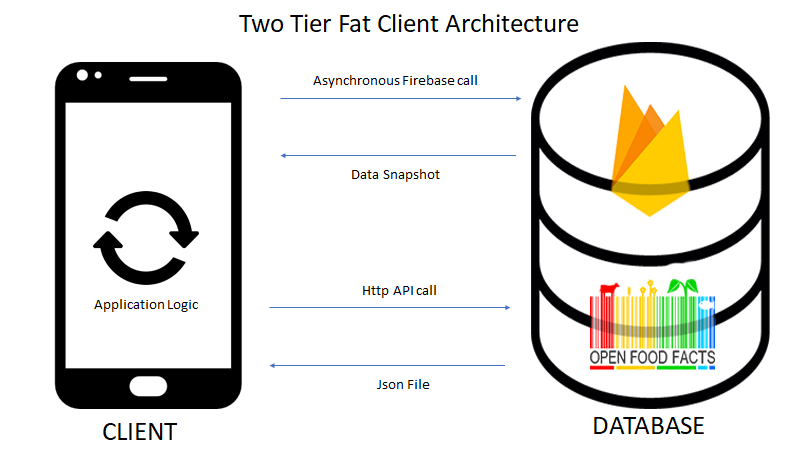
\includegraphics[height=8cm, width=\linewidth]{ArchitectureTwoTier.png}
\caption{Structure Overview} 
\end{figure}
\\
Bealthy uses a two tier architecture with a fat client. The client tier and the business logic tier are both located within the mobile application, while the database is remote. Most of the data are in the database managed by the provider "Firebase" on which there are all the static data of the predefined dishes, the dishes created by the user, the day by day information of which dishes he eats and which symptoms he shows, and the files of the images of the dishes and the photo of the user. The other part of the data is managed by the provider "OpenFoodFacts", an open source database containing thousands of food information associated with a barcode.

\subsection{High level components}
The architecture of the high-level components consists of two different types of elements:
the External Services and the Mobile Application.
\begin{itemize}
\item \textbf{The Mobile Application} allows users to interact directly with the system. This component provides a simple and clear view of the various functions that the system provides to the user. We decided to develop a fat client application that handles both the UI and UX part as well as the business logic. A fat client application  connects to a external remote database (firebase) in order to sync data or upload and download user information. 
Bealthy processes most of data by itself, it does not rely on any servers for processing. 
The processing of user data, in order to showing the correlation between the symptoms and the ingredients, is done offline.
\item There are two different kind of \textbf{External Services} that the application uses: The database ones and the authentication ones.
The external databases,Firebase and OpenFoodFact, are interrogated by our application when it needs their updated data while the external authentication services are: Google, Github and Twitter.
\end{itemize}

\subsection{Component view}

\null
\vspace{\stretch{2}}
\begin{figure}[ht!]
\centering
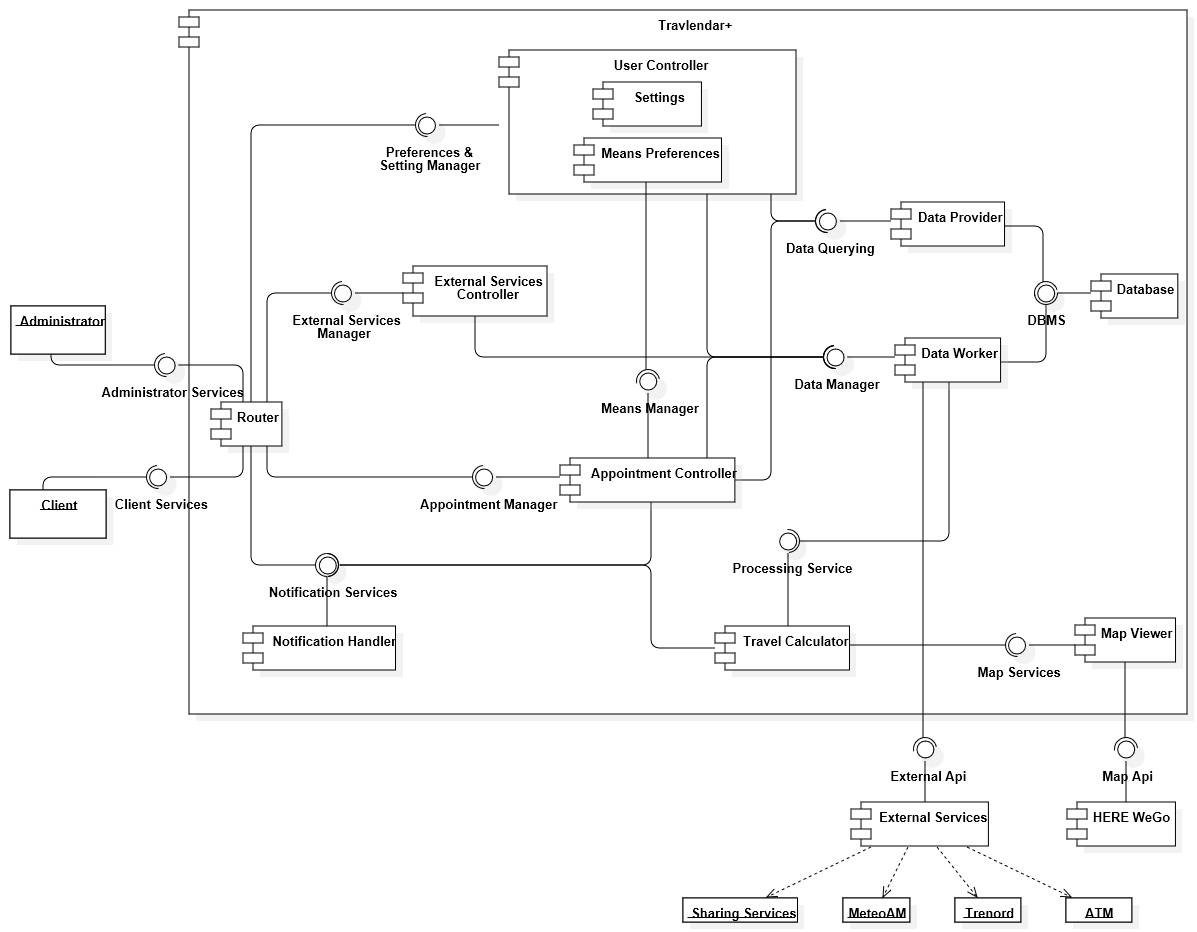
\includegraphics[height=14cm, width=\linewidth]{ComponentDiagram1.jpg}
\caption{Component Diagram}
\end{figure}  
\vspace{\stretch{5}}
\clearpage


\begin{itemize}[•]
\item Client:  the client’s device (mobile app).
\item Administrator: the administrator’s device (mobile app).
\end{itemize}
\clearpage

\subsection{Runtime view}
In the following Sequence Diagram for simplicity and clarity, some steps have been omitted in the communication between the components external to the main system and the router; as the main aspects of communication, between the User and the Travlendar system, have been dealt with in the RASD document.

\null
\vspace{\stretch{2}}
\subsubsection{Sequence Diagram 1}
This Sequence Diagram deals with the addition of an appointment by the customer. The request is taken on board by the router, which communicates with the appointments component and will show the user the form to fill in the data concerning his new event.\\
Subsequently, after the user has inserted the various information, the Appointment Controller component will check that it does not overlap with an existing one, in case the Notification Manager will send the user an error.\\
If the appointment is valid, the data worker will be asked to save the new appointment on the database and the latter will be responsible for providing the travel calculator with all the data necessary to calculate the trip from the previous position to that of the appointment, with the means and preferences that the user has selected.\\
If it is possible to solve the calculation, the travel itinerary will be saved and the user will receive a confirmation message; if not, it will be notified with a warning.
\vspace{\stretch{5}}
\\

\begin{figure}[ht!]
\centering
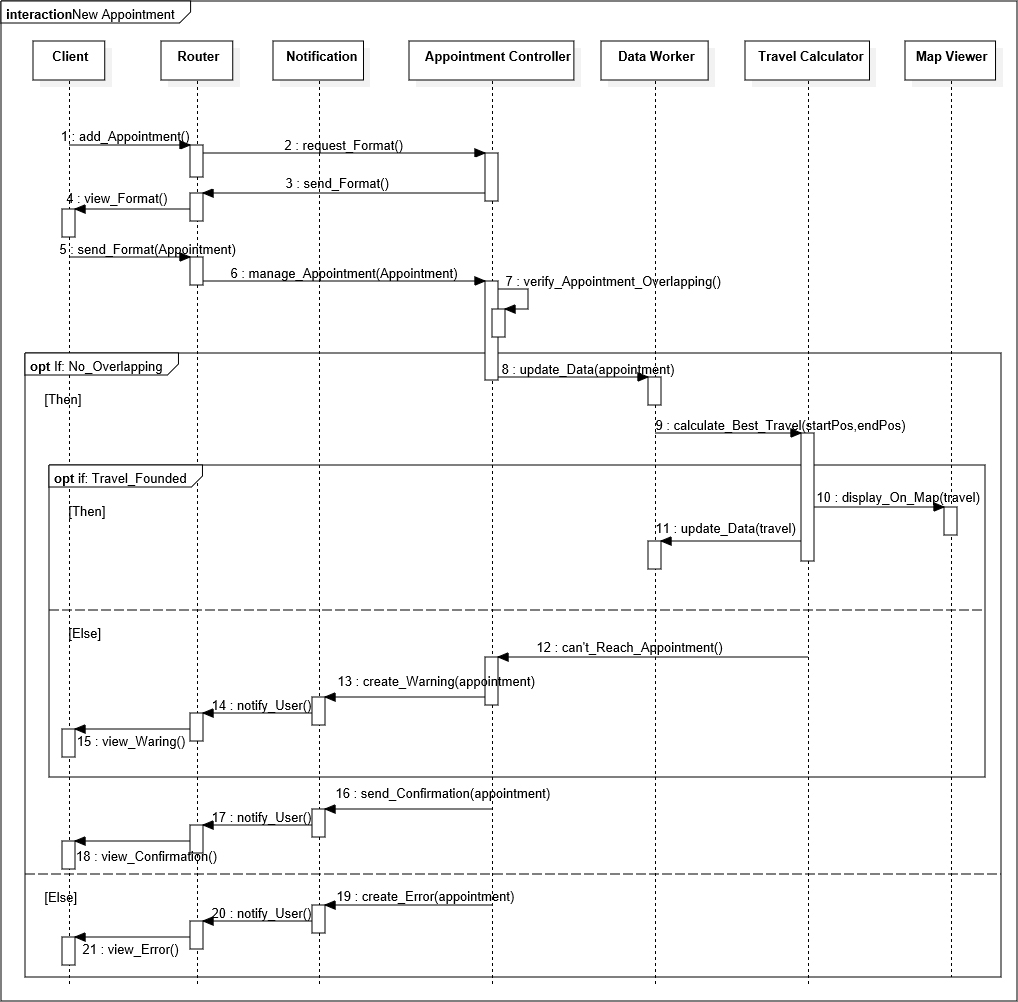
\includegraphics[height=19cm, width=\linewidth]{SQ1.jpg}
\caption{Sequence Diagram 1}
\end{figure}  
\clearpage



\subsection{Styles and patterns}
\subsubsection{Overall Architecture}

\begin{figure}[ht!]
\centering
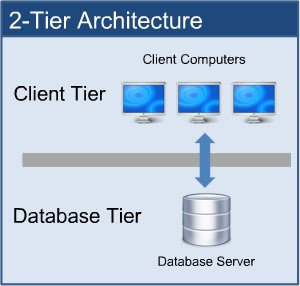
\includegraphics[height=7cm, width=7cm]{2tier.jpg}
\end{figure}  
Our application has been divided into 2 tiers: (fat client)
\begin{enumerate}
\item \textbf{Database tier ( DAL: Data Access Layer )}\\
Here information is stored and retrieved from an external database. The information is then passed to the logic tier for processing, and then eventually back to the user.
\item \textbf{Business Logic ( BLL: Business Logic Layer ) and Client tier (interface to BLL )} 
\\
The highest level of the application is the user interface, whose main function is to take care of all the user's requests, and to give him the possibility to interact quickly with the system.
The user will then be able to view own Symptoms, eaten dishes and statistics of a certain time period whenever he/she wishes.
Business Logic Tier is an important part of the Client Tier. 
It is managed by the "store" classes of our application through the use of \textbf{MobX} that is a state-management library that makes it simple to connect the reactive data of application with the UI.
All of these classes coordinate the application, process commands, make logical decisions and assessments and perform the calculations in order to elaborate user statistics chart of symptoms and ingredients. This level is mainly concerned with: processing the user's data and information, managing the interactions between our system and that of external Databases services.
\end{enumerate}
\clearpage

\subsubsection{Design decisions and patterns}
\begin{itemize}
\item We decided to use \textbf{Flutter} because it is Google’s UI toolkit used for building natively compiled applications for mobile from a single codebase. It is characterize by a fast development that allow to
use a rich set of fully-customizable widgets in order to build native interfaces.
\item Flutter provides a lot of flexibility in deciding how to organize and architect your apps. We decided to use the library \textbf{MobX} because it is a popular state management library for Dart and Flutter apps. It has also been recognized as a Flutter Favorite package.
MobX relies on 3 core concepts: Observables, Actions and Reactions. Observables represent the reactive state of your application. Actions are semantic operations that modify these observables and Reactions are the listeners that "react" to the change in Observables, by updating UI or firing network operations. Reactions are considered as the side-effects in a MobX-based application.
\begin{figure}[ht!]
\centering
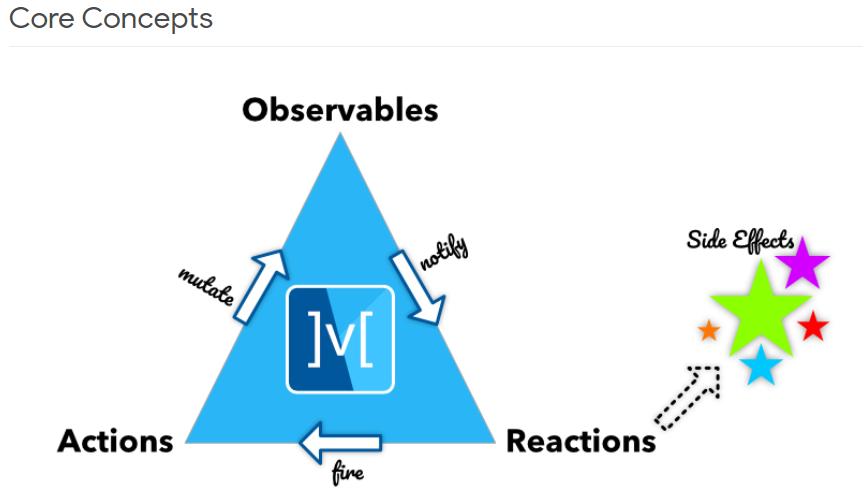
\includegraphics[height=7cm, width=12cm]{MobX.png}
\end{figure}

\end{itemize}
\section{Algorithm design}

\subsection{Brief description of the best travel calculation algorithm}

\subsection{Software System Attributes} 

\subsubsection{Reliability}
The users age range is 16-40 years old, so the system will be designed to be always reliable:
\begin{itemize}
\item On workday, in the early morning (7-10) and in the late afternoon (16-19); 
\item On weekend, from the midday to middle evening (11-16) and in the evening (19-24);
\end{itemize}
Because during the working day the user will use the application mainly for register his working or studying appointment and some personal engagements.\\
While in the weekend the user will register his leisure events and night friends meeting.

\subsubsection{Availability}
The system must guarantee a 24/7 service. Very small interrupt of the service during the day will be acceptable and tolerated. But when an issue occurs, the system must respond correctly after a maximum of 3 user attempts.
\subsubsection{Security}
Users credentials and external services account will be cryptate and stored in a reserved and protect area of the system database. Also, the privacy information about the user movement and his localization must be all encrypted and totally protected.
\subsubsection{Maintainability}
Our system uses many external APIs, so the maintainability of our software is very much dependent on this factor. Our system must always be updated with external API interfaces, and it must always be able to interpret and exploit the data it obtains from them.
Generally, there should not be too much invasive maintenance processes, as it uses very popular APIs used by many other software, whose changes are often minimal and well documented.
\subsubsection{Portability}
The system in terms of portability shall be very flexible. The application logic and the system interfaces are abstractly separated; so, the application porting consist only in the re-adapting of the user interface with the new operating system.
Also, could be necessary to reimplement some of the system interaction with the external services.\\

\section{User Interface Design}


\section{Implementation,Integration and Test Plan:}
\subsection{Elements to be integrated}

\subsection{Integration Testing Strategy}

\subsection{Component Integration}

\subsection{Used Tools}
\begin{itemize}
\item StarUml 2.8.0
\item Miktex 2.9.6361
\item Texmaker 5.0.2
\item DeepL
\item GitHubDesktop 1.0.6
\item AdobePhotoshop CC 2017
\item Power Point
\end{itemize}
\end{document}